\documentclass{article}
\usepackage{amsmath}
\usepackage{amssymb}
\usepackage{graphicx}
\usepackage{lipsum}
\usepackage[margin=1in, includefoot]{geometry}
\usepackage{fancyhdr}
\usepackage{float}
\usepackage{subcaption}
\pagestyle{fancy}
\fancyhead{}
\fancyfoot{}
\fancyfoot[R]{ \thepage\ }
\renewcommand{\headrulewidth}{0pt}
\renewcommand{\footrulewidth}{0pt}
\begin{document}
\begin{titlepage}
	\begin{center}
	\huge{\bfseries Classification of Wines using FTIR Spectrum Analysis}\\
	\line(1,0){300}\\
	[0.1in]
	\textsc{\LARGE Winter in Data Science} \\
	\textsc{\large Analytics Club and DAV Team, IIT Bombay}\\
	[3cm]
	\textsc{\Large 
	Mentors :\\ 
	[-0.3cm]
	Samuel Raja Bethala \& Vanshika Sindhu}\\
	[8 cm]
	\end{center}
	\begin{flushright}
	\textsc{\Large Yash Mehta}\\
	\textsc{\large
	22B1504\\
	UID : 07\\
	14 January, 2024}\\
	\end{flushright}	
\end{titlepage}
\tableofcontents
\thispagestyle{empty}
\cleardoublepage
\setcounter{page}{1}



\section{INTRODUCTION}\label{sec:intro}
\textbf{Fourier Transform Infrared} (FTIR) spectroscopy is a powerful analytical technique widely employed in various scientific disciplines to investigate the molecular composition of materials. This spectroscopic method utilizes the interaction of infrared radiation with matter, providing valuable insights into the vibrational modes of molecules. The key advantage of FTIR spectroscopy lies in its ability to rapidly collect a broad spectrum of information, allowing for the identification of functional groups and the characterization of chemical structures.\\
\newline
In FTIR spectroscopy, a sample is exposed to infrared light, leading to the absorption, transmission, or reflection of specific wavelengths corresponding to the vibrational frequencies of molecular bonds. The resulting spectrum, generated through Fourier transformation of the raw data, offers a detailed fingerprint of the sample's chemical composition. FTIR has found widespread applications in diverse fields, including chemistry, biology, pharmaceuticals, and materials science, making it an indispensable tool for qualitative and quantitative analysis.\\ 
\newline
This project deals with the usage of FTIR spectra of 37 wine samples to classify them into two classes using K-Means Clustering.\\ 
[2cm]

\section{ABSTRACT}\label{sec:abstract}
The dataset comprises FTIR spectra from 37 red wines, with each bottle contributing three spectra, resulting in a total of 111 spectra. This dataset was sourced from a GitHub repository [1]. The wines were sampled in triplicate, and the FTIR spectra, obtained through \textbf{Attenuated Total Reflectance} sampling in the mid-infrared range, were collected randomly over multiple days.\\
\newline
The assertion is that among the 37 red wines, 19 are Cabernet Sauvignon, while the remaining 18 are Shiraz. However, the specific assignment of each wine to these categories is unknown.\\
\newline
The objective of this project is to employ an unsupervised classification algorithm, specifically K-Means Clustering, to categorize these 37 wines into the two proposed classes. The coding for the same is done using Python programming language with the help of Numpy, Pandas, Matplotlib and Scikit-Learn packages. The Jupyter Notebook is uploaded on a Github Repository [2].\\


\newpage

\section{DATA ANALYSIS, PRE-PROCESSING AND DIMENSIONALITY REDUCTION}
\subsection{Data Analysis}
The plots of spectra of all the samples were plotted. Three major peaks were observed. The following figure shows a plot of one of the samples, along with the three important peaks.

\begin{figure}[H]
	\centering 
	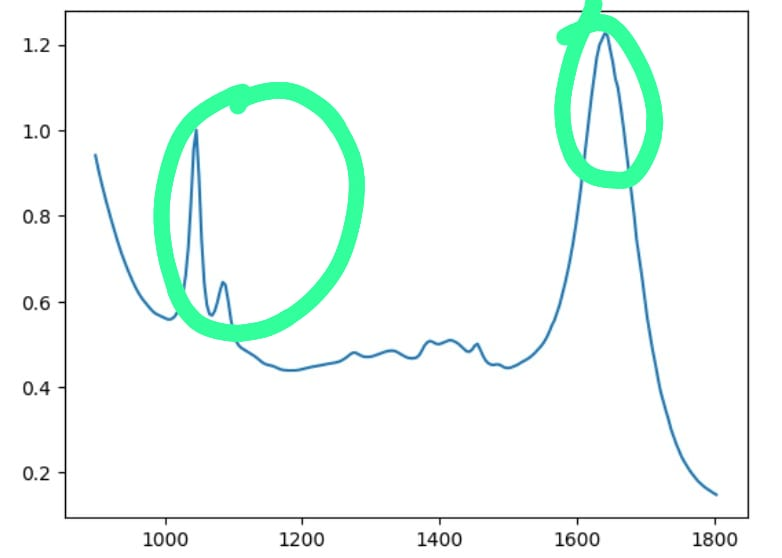
\includegraphics[height = 3in]{Three important peaks.jpeg}
	\caption[Optional Caption]{FTIR Spectrum of a wine sample along with three important peaks}
	\label{fig:fig1}
\end{figure}

\subsection{Data Pre-Processing}
The vector of each spectrum was re-scaled using \textbf{MinMaxScaler} function of \textbf{sklearn.preprocessing} package. This re-scales all the data points of the vector into a new value between 0 and 1 corresponding to the position of its original value with respect to the maximum and minimum values of that vector.\\
\newline
However, before scaling, a new dataframe was formed by excluding the data for wavenumbers less than 1000 and greater than 1750 from the original dataframe. This was done to restrict our attention to the three peaks.\\
\newline
Further, after scaling, a threshold was imposed on the dataframe to reduce those values which are less than that threshold, to zero. This was done to further restrict the data to the peaks.\\
\begin{figure}[H]
	\centering
	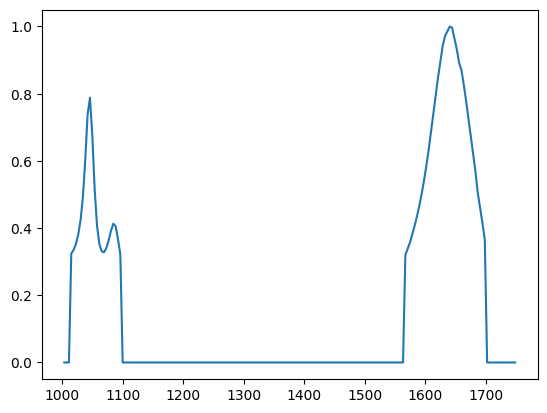
\includegraphics[height=3in]{Pre-processed Image.png}
	\caption[Optional Caption]{FTIR spectrum of a wine sample for a threshold of about 0.32}
	\label{fig:fig2}
\end{figure}

\subsection{Dimensionality Reduction}
Principal Component Analysis was used to reduce the number of features (i.e., the number of wavenumbers) from about 195 to 20-30. PCA was carried out using the PCA function of sklearn.decomposition package. Above 99\% of variance was captured in the new reduced dimensions. The dataset with reduced dimensions was stored in a new dataframe.\\
\newpage

\section{DATASET OF AVERAGE SPECTRA}\label{sec:rule}
Another dataset was made which had the average value of 3 intensities for each wavenumber for each wine. As a result, the new data set had 37 rows with each row containing the average spectrum of a wine. All the analyis, pre-processing and dimensionality reduction was done for this dataset as well. The purpose of this dataset was to compare the results of K-Means Clustering on both the data-sets to find the optimal value of the threshold. At this optimal value, the results of clustering on both the data-sets must match and the classification must be such that one of the classes must contain 19 wines and the other must contain the remaining 18.\\
\newline
Upon the application of K-Means Clustering, the resulting classes will be denoted as '0' and '1'. Given that the initial dataset included all three spectra of each wine in sequential order, it is imperative that, when classifying a particular wine, all three consecutive observations pertaining to that wine are assigned to the same class. In cases where two out of the three spectra share a common label and the third one differs, the majority's classification will be adopted for the entire set of three observations corresponding to that particular wine.\\
\newline
For example,\\
0 0 0 1 1 1 means that first wine belongs to class 0 and second belongs to class 1.\\
1 1 0 0 1 0 means that first wine belongs to class 1 and second wine belongs to class 0.\\
\begin{figure}[H]
	\centering 
	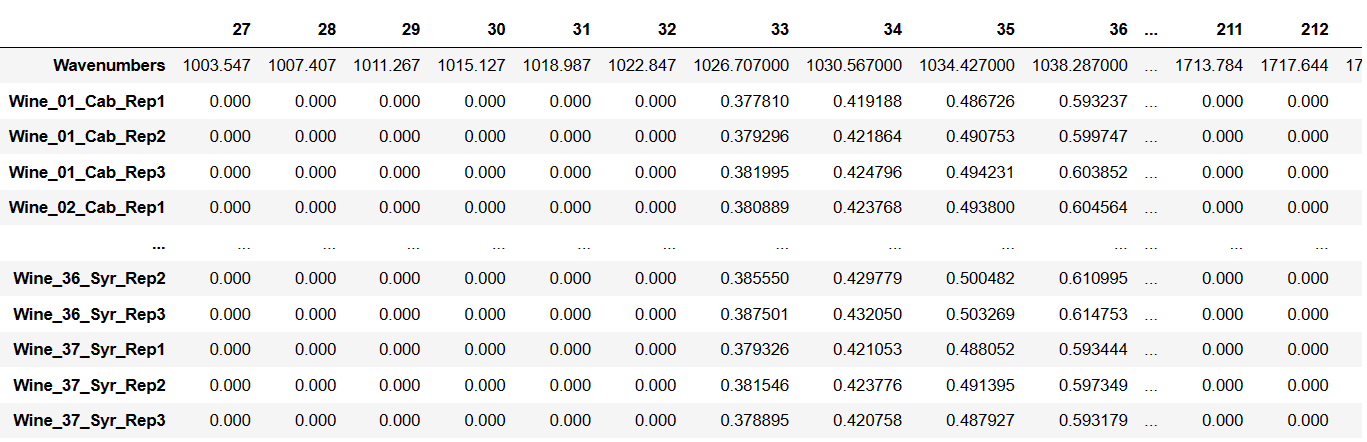
\includegraphics[height=1.5in]{Original Dataset.png}
	\caption[Optional Caption]{Figure of Original Dataset}
	\label{fig:fig3}
\end{figure}

\begin{figure}[H]
	\centering 
	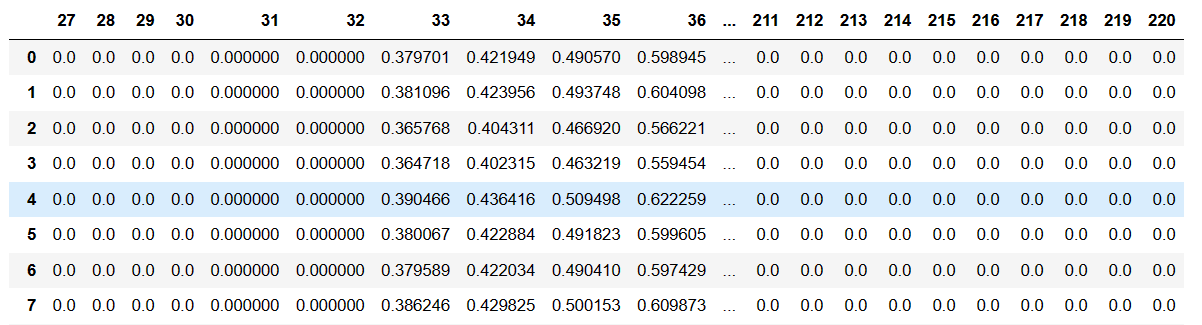
\includegraphics[height=1.5in]{Averaged Dataset.png}
	\caption[Optional Caption]{Figure of Dataset with Averaged Spectra}
	\label{fig:fig4}
\end{figure}
\newpage
\section{K-MEANS CLUSTERING}
K-Means Clustering is an unsupervised classification ML algorithm. Elbow method was applied on both the datasets to find the optimal number of 'k' (which is the number of clusters). To apply the elbow method, a new function 'optimize\textunderscore k\textunderscore means' was defined, which plots the graph of SSE for different k-values. The k-value (known as the optimal k-value) where the elbow occurs in the graph is selected. \\
\newline
The optimal k-value is expected to come out to be 2 for both the datasets. After this, the K-Means Clustering algorithm is applied to both the datasets for k=2 for different values of the threshold.\\
\begin{figure}[H]
	\centering
	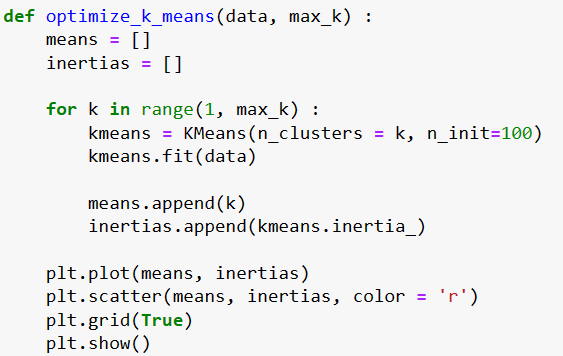
\includegraphics[height=2in]{Optimize k means.png}
	\caption[Optional Caption]{'optimize\textunderscore k\textunderscore means' function} 
	\label{fig:fig5}
\end{figure}
\subsection{Impact of Threshold on the Optimal K-Value and Predicted Clusters}
The main purpose of this project was to classify the 37 wines into two classes (one of 19 and other of 18). For that, two types of datasets were used (one being the original dataset and the other being the dataset of average spectra). The threshold was applied on both the datasets to control the amount of data from both the datasets being used for clustering. The main aim was to find such values of threshold for both the datasets that the optimal k-value for both the datasets came out to be 2 and the clustered wines from both the datasets matched at the end. \\
\newline
To achieve this, the K-Means Clustering algorithm was tested for a variety of thresholds for both the datasets. It was but obvious that the optimal thresholds for both the datasets would not differ much.\\
\subsection{The Optimal Threshold and the Resulting Clusters}
After a series of trials and errors, it was observed that at threshold = 0.3595 for the original dataset and 0.35925 for the dataset of average spectra, the resulting predicted clusters were - \\
\begin{figure}[H]
	\centering
	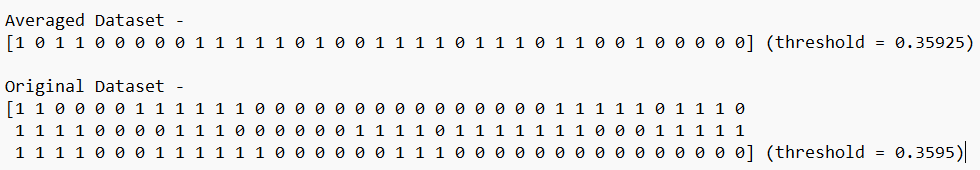
\includegraphics[height=1in]{Thresholds .png}
	\caption[Optional Caption]{Optimal values of threshold}
	\label{fig:fig6}
\end{figure}
It can be seen from the figure \ref{fig:fig6} by using the rule described in section \ref{sec:rule} that for the optimal values of threshold, the wines classified into 2 clusters almost match for both the datasets. \\
\newline
It also observed that the optimal value of k for these thresholds is 2.\\  
\newline
Let us now see the results pictorially.\\
\begin{figure}[H]
\centering
\begin{subfigure}{0.5\textwidth}
\centering
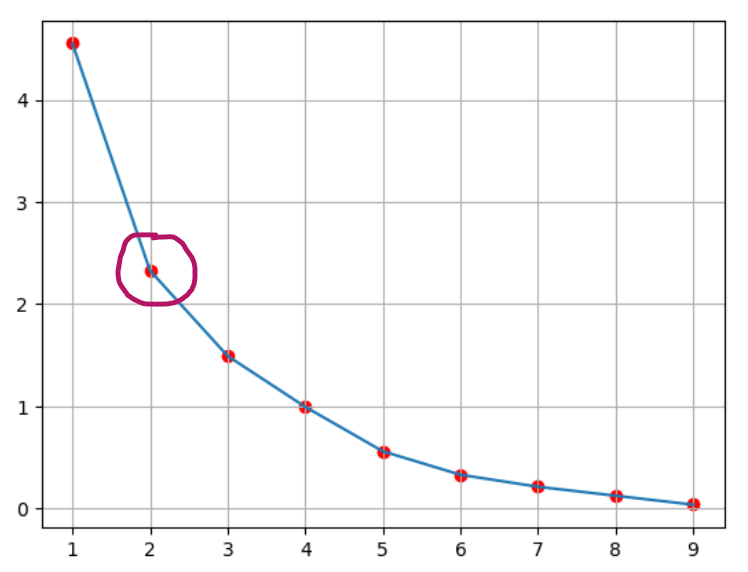
\includegraphics[height=1in]{Optimal k for avg dataset.png}
\caption[Optional Caption]{Elbow for Averaged Dataset}
\end{subfigure}%
\begin{subfigure}{0.5\textwidth}
\centering
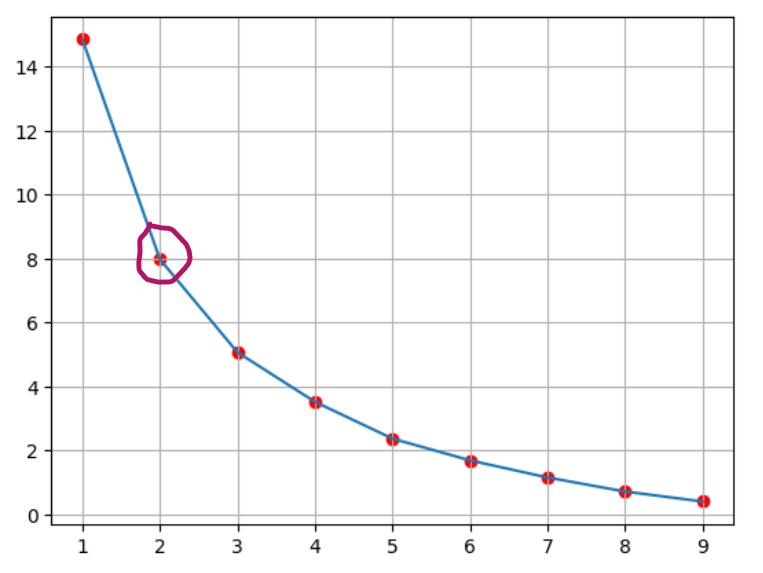
\includegraphics[height=1in]{Optimal k for og dataset.png}
\caption[Optional Caption]{Elbow for Original Dataset}
\end{subfigure}
\caption[Optional Caption]{Optimal K-Values}
\end{figure}


\begin{figure}[H]
\centering
\begin{subfigure}{0.5\textwidth}
\centering
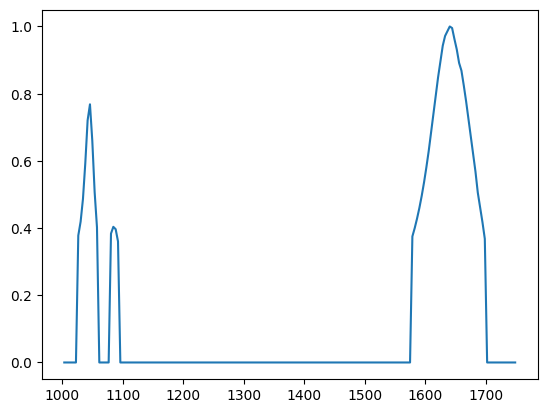
\includegraphics[height=2in]{Original Dataset optimal image.png}
\caption[Optional Caption]{A Spectrum from Original Dataset \\after applying Optimal Threshold}
\end{subfigure}%
\begin{subfigure}{0.5\textwidth}
\centering
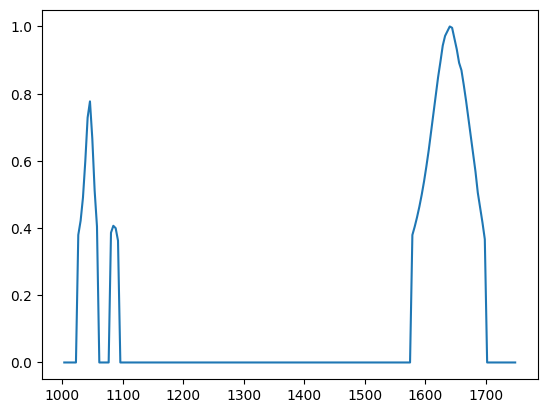
\includegraphics[height=2in]{Avergaed Dataset optimal image.png}
\caption[Optional Caption]{A Spectrum from Wine Sample from Averaged Dataset \\after applying Optimal Threshold}
\end{subfigure}
\caption[Optional Caption]{Optimal Thresholds applied on Graphs}
\end{figure}


\newpage
\section{CONCLUSION AND REFERENCES} 
\subsection{Conclusion}
The 37 wines were successfully classified into two classes. For this, two datasets were used - the original dataset and the data set with the averaged spectra. This was done to compare the results of K-Means Clustering for both the datasets and to find the optimal threshold for both the datasets at which all the 37 wines are classified into the required two classes with one class having 18 wines and the other having 19 wines. The threshold was applied to restrict the input data to the three significant peaks of the wine samples. \\
\newline
The optimal threshold value come out to be 0.3595 for the original dataset and 0.35925 for the averaged dataset, for which the results of clustering on both the datasets match.\\
\newline
The classes of 37 wines are as follows - \\
1 0 1 1 0 0 0 0 0 1 1 1 1 1 0 1 0 0 1 1 1 1 0 1 1 1 0 1 1 0 0 1 0 0 0 0 0\\
where 1 denotes the class with 19 wines \\
and 0 denotes the class with 18 wines.\\
\subsection{References}
[1] Github Repository for Dataset - https://github.com/QIBChemometrics/Wine\textunderscore Cabernet\textunderscore Shiraz\textunderscore FTIR/tree/main
[2] Github Repository for Python Code of this project - https://github.com/YashMehta25/WiDS\\
/blob/main/WiDS\%20Project.ipynb
\end{document}